\section{Aufbau}
\label{sec:Aufbau}
Der Aufbau ist in \autoref{fig:Aufbau} dargestellt.
\begin{figure}[H]
    \centering
    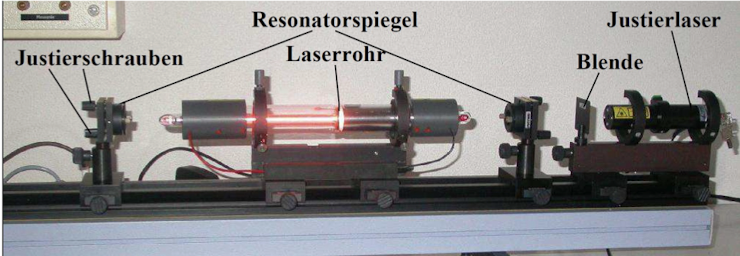
\includegraphics[scale=0.7]{Abbildungen/Aufbau.png}
    \caption{Bild vom Versuchsaufbau.\cite{V61}}
    \label{fig:Aufbau}
\end{figure}
Der Versuchsaufbau besteht hauptsächlich aus einer optischen Schiene, auf welcher verschiedene Bauteile montiert werden können.
Auf der rechten Seite befindet sich ein Justierlaser, welcher ausgerichtet werden muss. Dafür kann ein Schirm mit Fadenkreuz und eine Beugungsblende
jeweils direkt hinter dem Justierlaser und am Ende der optischen Bank positioniert werden. Der Justierlaser ist richtig ausgerichtet, wenn die 
Beugungsringe direkt im Fadenkreuz liegen.\\
Der eigentliche Laser besteht aus einem Laserrohr und zwei hochreflektierenden Spiegeln.
Es gibt verschiedene Spiegel, die ausgetauscht werden können. Diese bilden den Laserresonator.
Das Laserrohr ist mit einem Gasgemisch aus Helium und Neon gefüllt und mit Elektroden versehen. Dadurch kann, mittels Gasentladung eine Besetzungsinversion stattfinden.
Damit eine definierte Polarisationsrichtung gewährleistet wird, befinden sich am Ende der Laserröhre Brewster-Fenster.\\
In den Strahlengang können verschiedene Komponenten eingefügt werden, um die Lasereigenschaften zu untersuchen.

\section{Durchführung}
\label{sec:Durchführung}
Im Folgenden wird die Durchführung in die unterschiedlichen Messprogramme unterteilt.

Vor den Messungen wird kontrolliert ob der Justierlaser ausgerichtet ist. Dies ist daran zu erkennen, dass die Fadenkreuze in der Mitte der Beugungsringe
liegen.
Es wird der Justierlaser ausgestellt und der Strom der Hochspannung
auf $I = \qty{6.5}{\milli\A}$ eingestellt. Die Lasertätigkeit wird eingestellt, indem an den Justierschrauben der Resonatorspiegel
nachjustiert wird.


\subsection{Stabilitätsbedingung überprüfen}
\label{subsec:Stabilitätsbedingung}
Der Laser wird mit der Photodiode auf die maximale Leistung einjustiert.
Anschließend wird der maximal mögliche Resonatorabstand eingestellt, indem der Abstand der beiden Laserspiegel, bei laufendem Laser, vergrößert wird.
Dabei muss die Laserleistung nachjustiert werden.
Diese Messung wird analog für eine weitere Kombination der verfügbaren Spiegel durchgeführt.

\subsection{Beobachten von TEM-Moden}
\label{subsec:Moden}
Es sollen möglichst viele Moden stabilisiert und identifiziert werden. Zwischen den Resonatorspiegel und das Laserrohr
wird ein Wolframdraht, mit einer Dicke von $d = \qty{0.005}{\milli\meter}$, gebracht und verschoben. Dieser wird zur Stabilisierung
der Moden benutzt, indem der Draht so verschoben wird, dass verschiedene Moden auf dem optischen Schirm erkennbar sind.
Zur Erkennung der Moden wird der Strahldurchmesser des Lasers mit Hilfe einer Streulinse vergrößert. Zur Messung der Moden wird der optische Schirm mit 
einer Photodiode ersetzt. Es werden zwei Moden vermessen.

\subsection{Bestimmung der Polarisation}
\label{subsec:Polarisation}
Es wird ein Polarisator hinter den Auskopplungspiegel gestellt und die Intensität mit einer Photodiode gemessen.
Die Polarisationsrichtung wird stetig verändert.

\subsection{Der Multimodenbetrieb und das Frequenzspektrum des Lasers}
\label{subsec:Multimodenbetrieb}
Zur Untersuchung des Multimodenbetriebs wird die Schwebungsfrequenz vermessen, indem eine schnelle Photodiode, mit einer Bandbreite
von $\qty{1}{\giga\Hz}$, benutzt wird um die Frequenzen zu messen. Mittels eines Spektrumanalysators werden die Fourierspektren für 
unterschiedliche Resonatorlängen untersucht.

\subsection{Bestimmung der Wellenlänge}
\label{subsec:Wellenlänge}
Die Wellenlänge wird mit den Beugungsmaxima verschiedener Gitter bestimmt, die in den Strahlengang gestellt werden.